\documentclass[journal]{IAENGtran}

\ifCLASSINFOpdf
   \usepackage[pdftex]{graphicx}
   \DeclareGraphicsExtensions{.pdf,.jpeg,.png}
\else
   \usepackage[dvips]{graphicx}
   \DeclareGraphicsExtensions{.eps}
\fi

\begin{document}
\title{An Explanation Method of Unfamiliar Tourist Spots based on Roles of User's Familiar Spots}
\author{Kenta~Han and Daisuke~Kitayama

\thanks{K. T. Han is with the Graduate School of Engineering, Kogakuin University, Japan; e-mail: em18011@ns.kogakuin.ac.jp.}% <-this % stops a space
\thanks{D. Kitayama is with the Faculty of Informatics, Kogakuin University, Japan;  e-mail: kitayama@cc.kogakuin.ac.jp.}}% <-this % stops a space

\maketitle

\pagestyle{empty}
\thispagestyle{empty}

\begin{abstract}
Most tourists resort to available information online when planning for leisure travel; however, this recourse often becomes problematic and misleading as users of the information may be directed to unfamiliar areas. On this regard, we proposed a method of explaining unfamiliar spots through the familiar features of spots they have visited. We generated a feature vector using  tourist reviews of the tourist spot, then compared the vector with already visited spots to extract their role for guiding the user. Finally, we associated the visited spot with the unfamiliar spot by the similarity of the relative feature vector, and further extracted keywords that explain the relation. Furthermore, we developed a prototype of the system and evaluated the effect of the explanatory information between the familiar and unfamiliar spots.
\end{abstract}

\begin{IAENGkeywords}
Tourist spots, explainability, tourist reviews, paragraph vector
\end{IAENGkeywords}

\IAENGpeerreviewmaketitle

\section{Introduction}
\label{sec:Introduction}
\IAENGPARstart{T}{ourists} often resort to web information when planning travel destinations. The accuracy of these published guides is oftentimes unreliable and leads to the high probability of the traveler getting lost in an unfamiliar area. At present, most tourists read online reviews, travel and leisure communities ranking, and search engine recommendations regarding the spots they consider visiting. For instance, popular Japanese tourist spot posting sites Tripadvisor\footnote{https://www.tripadvisor.com/} and Jalan\footnote{Jalan https://www.jalan.net/kankou/} offer a wealth of information on destination reviews and experiences from travelers. Given that the potential traveler is unfamiliar to these spots, extracting the accurate location and information from the discussions and reviews might be a rigorous task. As an alternative, we proposed an effective locator technique for an unfamiliar spot using a spot visited and familiar to the user. This approach is analogous to employing experience over the current problem. To elucidate further, the previous experience indicates the already visited and familiar spot and the current problem is the unfamiliar spot. For instance, unfamiliar spots such as ``Omotesando'' in Tokyo, Japan may be located and understood easier by a newcomer French user when it is described as ``Avenue des Champs-Elysees'' in Paris, given that he/she has visited and is familiar with the latter area.
   In the proposed method, the user inputs already visited and unfamiliar spots. From this, a feature vector is generated based on user reviews of the tourist spot, and the relative feature vector is used for comparison with already visited spots to extract their role for the user. Finally, the visited spot is associated with the unfamiliar spot by similarity of their relative feature vector, and keywords that explain the relation are further extracted. This way, we aim to enhance user understanding of unfamiliar spots. Figure \ref{fig:Photo_Image} shows the concept of the proposed method.
   The rest of the paper is structured as follows. Section \ref{sec:Related Work}, introduces related works on the concept, while Section \ref{sec:An Explanation Method of Unfamiliar Tourist Spots} describes the method. Evaluation experiments and their results are discussed in Section \ref{sec:Evaluation Experiment}. Finally, Section \ref{sec:Conclusions and Future Work}, presents the conclusions of the paper and our future work.

\begin{figure}[t]
  \begin{center}
    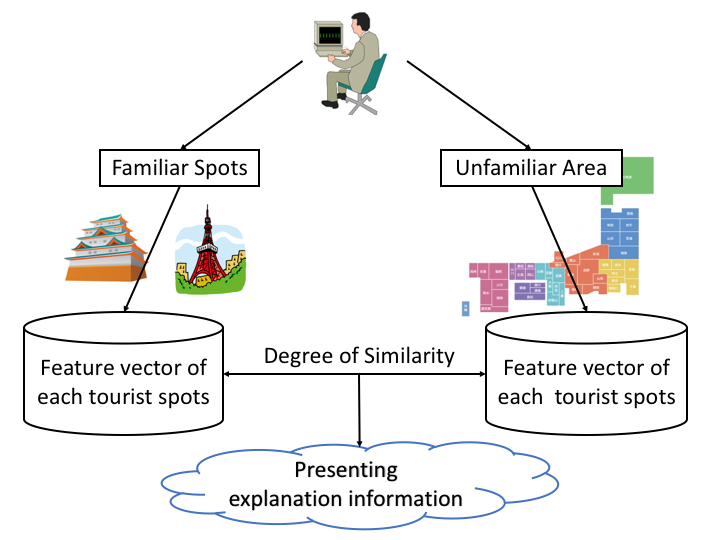
\includegraphics[clip,width=7.5cm,bb=0 0 720 540]{picture/Photo_Image_eng.png}
    \caption{An explanation method of unfamiliar tourist spots based on roles of user's familiar spots}
    \label{fig:Photo_Image}
   \end{center}
\end{figure}

\section{Related Work}
\label{sec:Related Work}
\subsection{Tourist spot retrieval and recommendation system}
\label{subsec:Tourist spot retrieval and recommendation system}

   Several research on retrieval and recommendation system using user's experience history have been published. Kurashima et al.\cite{Codd01} proposed a travel route recommendation method using geotag information of aggregated photos posted at Flickr, which could be regarded as personal travel history when sorted by time information. In this method, moving from a user's present location to a place easily accessible to his/her interest was presumed, and a behavior model was generated using the geotag information. Kitamura et al.\cite{Codd02} recommended sightseeing spots by estimating user's preferences of travel plan from past personal travel photographs using a general object recognition system to acquire keywords of subject information taken from the photos. Moreover, he represented the co-occurrence of the keywords by a graph visualization technique, which presents a user interface that visualizes a graph with travel photos. Conversely, Cheng et al.\cite{Codd03} used photographs of freely available community contributions to focus on personalized trip recommendations, considering suggested specific user profiles or attributes.

\subsection{The analogy and its applications}
\label{subsec:The analogy and its applications}
   Analogies were pointed out as contributing to creative thinking\cite{Codd04}; analogical thinking works when acquiring a concept (called the target) from known knowledge (called the bases)\cite{Codd05}. Many research on analogy were given the base learning data and targeted problems, and the problems were solved by mapping the features of things to the feature of the problem\cite{Codd06}. Gick et al. investigated the use of analogies between disparate domains as a guide to finding solutions for an ill-defined problem. Some studied on how to give learning data and functions\cite{Codd07}, and clarified whether to solve the problem depending on the degree of cognitive proficiency\cite{Codd08}. In many of the conventional research including these, after giving bases and targets for analogy, problems were solved according to a certain procedure. There are three types of structural similarities: ``similarity of object level'' determined by the number of shared features, ``relationship similarity'' based on the degree of sharedness of relationships existing in the base and the relationship existing in the base, and ``pragmatic similarity'' based on the title solution or target level \cite{Codd05},\cite{Codd09}.
   In the conventional method of using the user's experience history, several research analyzed the geotag information of the history photograph and converted them into user's preference; analogy techniques were also utilized to support learning and understanding. In this research, a review of familiar spots and unfamiliar spots and the relative features of each spot, via the sets of spots familiar and unfamiliar to the user, were determined and associated to enhance understanding of the area information. As it exploited analogy explicitly, this paper is presumed to have similar structure as with the "similarity of relationship level."

\section{An Explanation Method of Unfamiliar Tourist Spots}
\label{sec:An Explainaton Method of Unfamiliar Tourist Spots}

   In this method, the user inputs a set of tourist spots he/she has visited and the destination he/she intends to visit. Next, a feature vector is generated based on user reviews of the intended tourist spot. Afterwards, a feature vector relative to the visited spots is used for extraction of their role to the intended destination of the user. The relative feature vector of each tourist spot in the unfamiliar area is calculated and compared. Finally, the relative feature vector of the unfamiliar spot is associated to the similar feature vector of the visited spot, and the keywords explaining the relation are extracted.

\subsection{Generating feature vector using user reviews of spot}
\label{subsec:Generating feature vector using user reviews of spot}
   We used the review data obtained from ``Jalan'' until the end of September 2016. We generated feature vectors of tourist spots using paragraph vector\cite{Codd10}; we combined all reviews on a tourist spot and treated them as one document. We used a Python library called gensim\footnote{https://radimrehurek.com/gensim/models/doc2vec.html} to calculate the paragraph vector, and the Distributed Bag-of-Words with 300 dimensions as the learning method. As user reviews in Jalan are written in Japanese, we used MeCab\cite{Codd11} as the Japanese morphological analyzer with dictionary ``mecab-ipadic-NEologd''\footnote{https://github.com/neologd/mecab-ipadic-neologd/}.

\subsection{Relative features for role of tourist spots}
\label{subsec:Relative features of tourist spots}

\begin{figure}[t]
  \begin{center}
    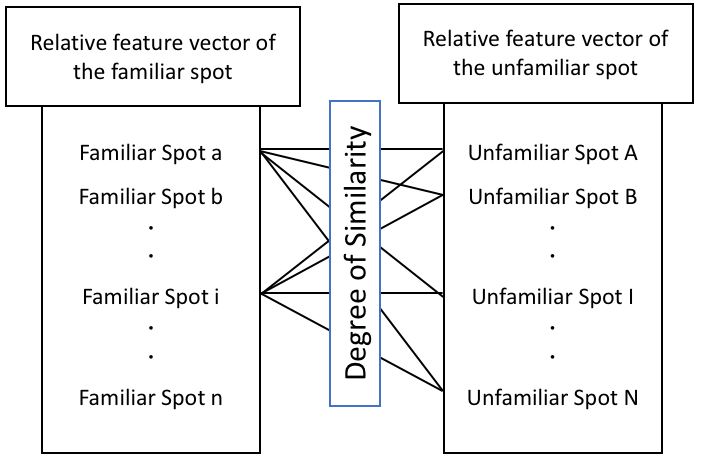
\includegraphics[clip,width=7.5cm,bb=0 0 720 540]{picture/Photo_CosSim_eng.png}
    % 類似度計算概念図
    \caption{Concept of similarity calculation}
    \label{fig:Photo_CosSim}
  \end{center}
\end{figure}

   We extracted the role of tourist spots by comparing their relative features with those of other tourist spots. A relative feature is defined here as the feature of the target spot that is compared to the average feature of a set of tourist spots. For example, we could consider ``the Tokyo Metropolitan Government Building Observatories (TMGBO)'' and ``Kinkakuji Temple'' under a set of famous tourist spots in Japan. The relative features of ``Kinkakuji Temple'' are the temple, its golden color, the city of Kyoto, and so on, while ``TMGBO'' has the features of panoramic view, night view, the building itself, the Shinjuku ward, and so on. When compared with other tourist spots, the relative features of the two examples tend to be general features, categories, and places.
   Let us take another example. We could consider ``Kinkakuji Temple'' and ``Kiyomizudera Temple'' under a set of temples in Kyoto, Japan. The relative features of ``Kinkakuji Temple'' are its golden color, gold leaf, brilliance, and so on, while for ``Kiyomizudera Temple'' these features include the stage, the panoramic view, and so on. As both temples are located in Kyoto, features related to Kyoto and temples do not appear as relative features; instead, more detailed features are obtained.
   The relative feature vector $r_{state,i}$  is obtained by subtracting the average of feature vectors of other spots from its own feature vector as in
\begin{equation}
  r_{state,i}=s_i-average(S_{state}-s_i),
  \label{math:Vector difference}
\end{equation}
where $S_{state} =\{s_1,s_2,\dots,s_n\}$ is a familiar spot set when $state$ is $'f'$; otherwise, it is an unfamiliar spot set when $state$ is $'f'$. The term $s_i$ is a feature vector of a tourist spot in the set $S_{state}$.

\subsection{Determination of an explainable spot}
\label{subsec:Determination of an explainable spot}
   We used a familiar spot to explain the spot in the unfamiliar area. We associated unfamiliar spots and familiar spots through the similarity calculated by the relative feature vector of the familiar spot $r_{f,i}$ and the unfamiliar spot $r_{u,j}$ (Fig. \ref{fig:Photo_CosSim} ). We used  the cosine scale below for the calculation
\begin{eqnarray}
  cos(r_{f,i},r_{u,j})=\frac{r_{f,i} \cdot r_{u,j}}{|r_{f,i}| \times |r_{u,j}|.}
  \label{math:CosSim}
\end{eqnarray}

   The association procedure is explained as follows. First, we associated a spot with the highest degree of similarity to a certain spot. If similarity falls below the threshold (0.125 in this paper) then no association is made. The result depends on whether the familiar spot having the highest degree of similarity to the unfamiliar spot is associated, or the unfamiliar spot having the maximum similarity to the familiar spot is associated. In the former condition, when all similarities have exceeded the threshold, all familiar spots, but not all unfamiliar spots, have corresponding spots. Conversely, in the latter case, when all similarities have exceeded the threshold, all unfamiliar spots have corresponding spots. To provide explanation for an unfamiliar spot, we adopted the latter condition.

\subsection{Extraction of explainable words for role}
\label{subsec:Extraction of explainable words for role}
   Keywords representing the viewpoints of association between the unfamiliar and familiar spots were presented to the user. However, as extracting the feature of a word from the relative feature vector was not possible, we resorted to another method. As a premise, all reviews were divided into words by the Japanese morphological analyzer MeCab, where we used ``mecab-ipadic-NEologd'' as the dictionary; however, the words particle, auxiliary verb, adnominal, symbol, and stop, were deleted. For the keyword extraction, we first obtained a feature word and tfidf value from the target familiar spot and unfamiliar spots by the tfidf method. Next, we calculated the harmonic mean of the tfidf values to score feature words common to the two spots. Finally, we extracted the feature words with high scores as explainable words.
   We calculated the feature value of a keyword in a spot by the formula
\begin{equation}
  TFIDF(t,d,state) = TF(t,d) \times log\Biggr(\frac{|S_{state}|}{DF(t,state),}\Biggr)
  \label{math:TFIDF}
\end{equation}
where function $TF(t,d)$ returns the number of the keyword $t$ in the document $d$, which combines all reviews of a spot into one; function $DF(t,state)$ returns the number of documents that include keyword $t$ and; $|S_{state}|$ is the total number of spots.
When $state$ was $f$, we calculated TFIDF using a set of familiar spots from the user spot inputs. Likewise when $state$ was $u$, we calculated TFIDF using the set of unfamiliar spots from the user area inputs.
   We extracted the explainable keywords of the associated familiar and unfamiliar spots using the harmonic mean of the TFIDF values of the feature words common to the two spots. First, we extracted words commonly appearing in the review document of the familiar and unfamiliar spots. Next, we calculated the score of the extracted word by formula \ref{math:Harmonic Mean}. $TFIDF(t,d,f)$ and $TFIDF(t,d,u)$ indicate the TFIDF value of the familiar and unfamiliar spots, respectively. The word has high importance in each spot when the score is large. Therefore, the top $N$ words of the score were presented as explanatory information to the user (Fig. \ref{fig:photo_map}).

\begin{eqnarray}
  score(t,d) = \frac{2 \times TFIDF(t,d,f) \times TFIDF(t,d,u)}{TFIDF(t,d,f) + TFIDF(t,d,u)}.
  \label{math:Harmonic Mean}
\end{eqnarray}

\begin{figure}[t]
  \begin{center}
    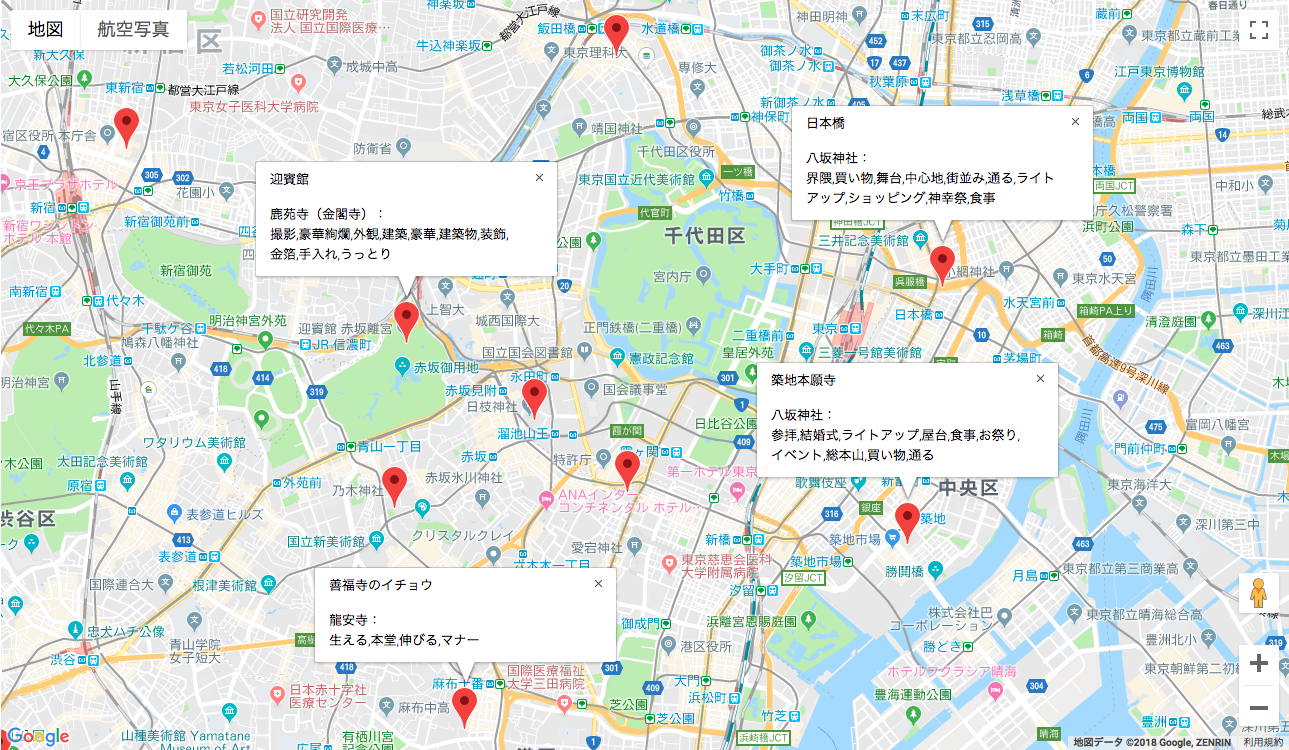
\includegraphics[clip,width=8.5cm,bb=0 0 1289 750]{picture/Photo_Map.png}
    \caption{User interface of prototype system}
    \label{fig:photo_map}
   \end{center}
\end{figure}

\subsection{Example of explained unfamiliar spots}
\label{subsec:Example of explained unfamiliar spots}

\begin{table}[t]
  \caption{Set of Familiar and Unfamiliar spot}
  \label{table:Familiar spot group and Unfamiliar spot group}
  \centering
  \begin{tabular}{l|l}
  \hline
  \multicolumn{1}{c|}{Familiar Spot Name} & \multicolumn{1}{c}{Unfamiliar Spot Name} \\ \hline
  Sensoji Temple                          & Tokyo Disneyland (R)                     \\
  Odawara-jo Park                         & Shinjuku Gyoen                           \\
  Fushimiinari-taisha Shrine              & Tokyo Skytree                            \\
  Nara Park                               & Tokyo Tower Main Deck            \\
  Mishima Skywalk                         & Meiji Jingu                              \\ \hline
  \end{tabular}
\end{table}

\begin{table*}[t]
  \caption{Explanation information}
  \label{table:Explanation information}
  \centering
  \begin{tabular}{l|l|l}
  \hline
  \multicolumn{1}{c|}{Unfamiliar Spot} & \multicolumn{1}{c|}{Familiar Spot} & \multicolumn{1}{c}{Explanation Information}                     \\ \hline
  Shinjuku Gyoen                      & Odawara-jo Park                         & flower viewing, bloom, inside the park, cherry-blossoms, leisurely, maintenance, nature, play equipment, azalea          \\
  Tokyo Skytree                     & Mishima Skywalk                    & Mt. Fuji, swing, high fear, ceiling, magnificent view, elevator, panorama, observation deck, rising
 \\ \hline
  \end{tabular}
\end{table*}

Table \ref{table:Familiar spot group and Unfamiliar spot group} shows an example of a set of user's familiar and unfamiliar spots. Five unfamiliar spots were randomly selected within Tokyo. Table \ref{table:Explanation information} shows the list of explainable words using the proposed method in Section \ref{sec:An Explanation Method of Unfamiliar Tourist Spots}.
   Focusing on the feature of the park, we believed that the spot closest to the park in the set of unfamiliar spots was ``Shinjuku Gyoen.'' In the set of familiar spots there were two parks, ``Odawara-jo Park'' and ``Nara Park.''
``Odawara-jo Park'' had many descriptions about flowers and play equipment, while ``Nara Park'' had many descriptions about deers and grasses. Because ``Shinjuku Gyoen'' had many descriptions about flowers and play equipment, it seemed related to ``Odawara-jo Park.''
   In the set of familiar spots, ``Mishima Skywalk'' had features of good view and high, while ``Tokyo Skytree'' and ``Tokyo Tower Main Deck'' had the same features in the set of unfamiliar spots. In this case, both could be considered as similar relative features. However, ``Mishima Skywalk'' was associated with ``Tokyo Skytree'' as the latter had a better view than ``Tokyo Tower Main Deck.'' Moreover, ``Mt. Fuji'' was extracted as an explainable keyword. A word that emphasizes the good view seemed to express the relationship appropriately. Thus, the proposed method can show the feature of each relationship.

\section{Evaluation Experiment}
\label{sec:Evaluation Experiment}
\subsection{Experiment settings}
\label{subsec:Experiment settings}
We compared the proposed method with these existing methods:
\begin{description}
\item[A.]Metadata (category, duration time, season)
\item[B.]Paragraph vector (feature vector)
\item[C.]Proposed Method (relative feature vector)
\end{description}
   Metadata (A) is used for searching spots on sightseeing spots search site. We selected three metadata that are often used:
\begin{itemize}
\item Category: e.g., shrine/temple,tourist facilities /tourist tours
\item Duration time: e.g., less than one hour,1--2 hours
\item Season: e.g., 1--12 month, spring, summer, autumn, winter
\end{itemize}
   In method A, familiar and unfamiliar spots of the same category, duration time, and season were extracted. If otherwise these could not be extracted, conditions in the order of season, duration time, and category were deleted
If there were multiple unfamiliar spots, we selected the one with the largest number of reviews. Moreover, we extracted the explainable words using Section \ref{subsec:Extraction of explainable words for role} and presented them to the subjects.
   Paragraph vector (B) uses the feature of each spot using the feature vector created in Section \ref{subsec:Generating feature vector using user reviews of spot}. For this method, we extracted the explainable words using Section \ref{subsec:Extraction of explainable words for role} and presented them to the subjects.
   We gathered 24 subjects using CrowdWorks\footnote{CrowdWorks is a crowdsourcing service in Japan. https://crowdworks.jp/} and presented them explainable information of unfamiliar spots based on their familiar spots using each method. The subjects inputted four to ten tourist spots they had visited and favored. In the system, to match the input character string with the spot name, the subjects selected from the spot list the candidates similar to the input character string. Afterwards, the subjects were asked to input destinations they intend to visit. We presented familiar and unfamiliar spots associated with methods A to C and their explainable keywords (N $\le$ 5).
The subjects evaluated the results by choosing one out of the following five options.
\begin{enumerate}
  \item No keyword.
  \item There is a relationship between the two spots, and the relationship became clear by keywords.
  \item There is a relationship between the two spots, and I noticed the relationship for the first time by keyword.
  \item There is a relationship between the two spots, but the keyword does not represent the relation.
  \item There is no relationship between the two spots.
\end{enumerate}

\subsection{Results}
\label{subsec:Results}

\begin{table}[t]
  \caption{Experimental results}
  \label{table:Statistics on the number of data of experiment results}
  \centering
  \begin{tabular}{c|r|r|r|r}
  \hline
  Evaluation & \multicolumn{1}{c|}{Method A} & \multicolumn{1}{c|}{Method B} & \multicolumn{1}{c|}{Method C} &  \multicolumn{1}{c}{Total} \\ \hline
  1  & 0                      & 0                      & 0                      & 4                      \\
  2  & 19                     & 44                     & 32                     & 121                    \\
  3  & 20                     & 62                     & 53                     & 191                    \\
  4  & 1                      & 3                      & 3                      & 10                     \\
  5  & 6                      & 21                     & 21                     & 68                     \\ \hline
  Total & 46                     & 130                    & 109                    & 285                    \\ \hline
  \end{tabular}
\end{table}

   Table \ref{table:Statistics on the number of data of experiment results} shows the experimental results for methods A to C. A total of 285 usable data were used in the experiment. As shown, method A had the smallest number of familiar spots associated with unfamiliar spots, while method B had the largest number of familiar spots related to unfamiliar spots.

\begin{table}[t]
  \caption{Percentage of evaluation in explanation information}
  \label{table:Percentage of evaluation in explanation information}
  \centering
  \begin{tabular}{c|r|r|r}
  \hline
  Evaluation & \multicolumn{1}{c|}{Method A} & \multicolumn{1}{c|}{Method B} & \multicolumn{1}{c}{Method C} \\ \hline
  1  & 0.00\%                     & 0.00\%                     & 0.00\%                                         \\
  2  & 41.30\%                    & 33.85\%                    & 29.36\%                                       \\
  3  & 43.48\%                    & 47.69\%                    & 48.62\%                                       \\
  4  & 2.17\%                     & 2.31\%                     & 2.75\%                                         \\
  5  & 13.04\%                    & 16.15\%                    & 19.27\%                                       \\ \hline
  \end{tabular}
\end{table}

\begin{table*}[t]
  \caption{Evaluation percentages when the categories of the familiar spots are different and when the familiar spots are similar}
  \label{table:When the categories different or similar}
  \centering
  \begin{tabular}{c|r|r}
  \hline
  & \multicolumn{1}{c|}{\begin{tabular}[c]{@{}c@{}}When the familiar spots are different\end{tabular}} & \multicolumn{1}{c}{\begin{tabular}[c]{@{}c@{}}When the familiar spots are similar\end{tabular}} \\ \hline
  Method B \& Option 2 & 56.82\%                            & 43.18\%                            \\
  Method C \& Option 2 & 71.87\%                            & 28.13\%                            \\ \hline
  Method B \& Option 3 & 51.61\%                            & 48.39\%                            \\
  Method C \& Option 3 & 52.83\%                            & 47.170\%                            \\ \hline
\end{tabular}
\end{table*}

   Table \ref{table:Percentage of evaluation in explanation information} shows the ratio of the number of the experimental results from options 1--5 in A to C. Most subjects chose option 2 for method A; this implied that A could associate spots having similar relationships. As for the proposed method (C), the ratio of option 2 decreased while it increased for option 3. This trend implied that method C found and presented hidden relationships. However, as the ratio of option 5 also increased, we could say that irrelevant spots were easier to extract.
   When options 2 and 3 were summed, method A had the highest explanation information percentage; therefore, it had the highest accuracy of association. However, as described above, option 2 is a natural relationship, and method A could extract only a small number. In our opinion, options 2 and 3 were observed to be in a trade-off relationship. Option 2 was a relationship that did not need bothersome explanation, while option 3 was a relationship worthy of explanation. We believe it important to increase choice 3 as much as possible while maintaining option 2. From this point of view, method B and the proposed method would show the same degree of accuracy.
   Option 3 had the high possibility of changing to option 5 if keyword extraction failed. Therefore, we would need to improve the method of keyword extraction.
   For methods B and C, the case where the category of the familiar spots inputted by the subject was different, was similar to the case where the categories of the familiar spots inputted by the subjects were different. Table \ref{table:When the categories different or similar} shows the ratio of the evaluation of options 2 and 3. With method C, which is the proposed method, subjects could present meaningful keywords without needing relation to a certain spot the subject has visited and is familiar with. Using the relative feature vector, the characteristics of each spot could be compared to using category. Furthermore, method B was better in the case where the genres of the familiar spots were similar.
\section{Conclusions and Future Work}
\label{sec:Conclusions and Future Work}

   We focused on the difficulty of understanding tourist spots suggested by search engines through ranking, visit recommendations, categories, and so on, given that these areas are unfamiliar to a web user. To support the understanding of unfamiliar spots by potential visitors, we proposed an explanatory method that compares the relative features of the spots in question and the areas they visited and are familiar with.
   We evaluated four methods, including our proposed method, for their accuracy on providing explanatory information. Using categories, the number of familiar spots associated with unfamiliar spots had the lowest accuracy. However, using relative feature vector and harmonic mean, the characteristics of each spot can be obtained. In addition, we confirmed it possible to correlate unexpected unfamiliar spots with familiar spots, and that there is a possibility that interest and attention can be drawn to tourist spots that users do not know.
   As future work, we intend to analyze the experimental results in terms of effectiveness and relevance of each keyword presented to the users.

\section*{Acknowledgment}
This work was supported by ISPS KAKENHI of Grant-in-Aid for Scientific Research(C) Grant Number 18K11551.

\ifCLASSOPTIONcaptionsoff
  \newpage
\fi

\begin{thebibliography}{1}
  \bibitem{Codd01}
    T. Kurashima, T. Iwata, G. Irie and K. Fujimura.,
      ``Travel route recommendation using geotags in photo sharing sites'',
      CIKM '10 Proceedings of the 19th ACM international conference on Information and knowledge management, pp.579-588, 2010
  \bibitem{Codd02}
    R. Kitamura and T. Itoh,
      ``Tourist Spot Recommmendation Applying Generic Object Recognition with Travel Photos'',
      ITE Tech. Rep., Vol.42, No.12, AIT2018-94, pp.185-188, 2018
  \bibitem{Codd03}
    A. J. Cheng, Y. Y. Chen, Y. T. Huang and Winston H. Hsu,
      ``Personalized Travel Recommendation by Mining People Attributes from Community-Contributed Photos'',
      MM '11 Proceedings of the 19th ACM international conference on Multimedia, pp.83-92, 2011
  \bibitem{Codd04}
    K. J. Holyoak and P. Thagard,
      ``Mental Leaps: Analogy in Creative Thought, MIT Press'',
      Journal of Japanese Society for Artificial Intelligence,  Vol.11, No.3,  pp.489, 1996
  \bibitem{Codd05}
    D. Gentner,
      ``Structure-Mapping: A Theoretical Framework for Analogy'',
      Cognitive Science, Vol.7, pp.155-170, 1983
  \bibitem{Codd06}
    M. L. Gick and K. J. Holyoak,
      ``Analogical Problem Solving'',
      Cognitive Psychology, Vol.12, pp.306-355, 1980
  \bibitem{Codd07}
    M. L. Gick and K. J. Holyoak,
      ``Scheme Induction and Similarity in Analogical Transfer'',
      Cognitive Psychology, Vol.15, pp.1-38, 1983
  \bibitem{Codd08}
    Z. Chen and M. W. Daehler,
      ``Positive and Negative Transfer in Analogical Problem-solving by 6-years-old Children'',
      Cognitive Development, Vol.4, No.4, pp.327-344, 1989
  \bibitem{Codd09}
    K. J. Holyoak and P. Thagard,
      ``Analogical Mapping by Constraint Satisfaction'',
      Cognitive Science, Vol.13, pp.295-355, 1989
  \bibitem{Codd10}
    Quoc V. Le and Tomas Mikolov,
      ``Distributed representations of sentences and documents'',
      In Proceedings of the 31th International Conference on Machine Learning, ICML 2014, pp. 1188-1196, 2014
  \bibitem{Codd11}
    T. Kudo, K. Yamamoto and Y. Matsumoto,
    ``Applying Conditional Random Fields to Japanese Morphological Analysis'',
    Proceedings of the 2004 Conference on Empirical Methods in Natural Language Processing (EMNLP-2004), pp.230-237, 2004

\end{thebibliography}
\end{document}
